\documentclass[sigconf]{acmart}

\newcommand{\FIXME}[1]{{\color{red}{\textbf{FIXME:}#1}}}

\usepackage{booktabs} % For formal tables

% Copyright
%\setcopyright{none}
%\setcopyright{acmcopyright}
%\setcopyright{acmlicensed}
\setcopyright{rightsretained}
%\setcopyright{usgov}
%\setcopyright{usgovmixed}
%\setcopyright{cagov}
%\setcopyright{cagovmixed}


% DOI
\acmDOI{10.475/123_4}

% ISBN
\acmISBN{123-4567-24-567/08/06}

%Conference
\acmConference[SHORTNAME'17]{ACM Long Conference Name conference}{July 1997}{City, State, Country} 
\acmYear{2017}
\copyrightyear{2017}

\acmPrice{15.00}


\begin{document}
\title{Tango: Dynamic Booster Coupling for Data Center Networks}
%\title{SIG Proceedings Paper in LaTeX Format}
%\titlenote{Produces the permission block, and copyright information}
%\subtitle{Extended Abstract}

\author{Anirudh Chelluri \kern1em
 Andre DeHon \kern1em
 Hans Giesen \kern1em
 Boon Thau Loo \kern1em
 Nishanth Prabhu \kern1em
 Lei Shi \kern1em
 John Sonchack \kern1em
 Nik Sultana}
\affiliation{%
\institution{University of Pennsylvania}}

%\author{Firstname Lastname}
%\authornote{Note}
%\orcid{1234-5678-9012}
%\affiliation{%
%  \institution{Affiliation}
%  \streetaddress{Address}
%  \city{City} 
%  \state{State} 
%  \postcode{Zipcode}
%}
%\email{email@domain.com}
%
%\author{Firstname Lastname}
%\orcid{1234-5678-9012}
%\affiliation{%
%  \institution{Affiliation}
%  \streetaddress{Address}
%  \city{City} 
%  \state{State} 
%  \postcode{Zipcode}
%}
%\email{email@domain.com}
%
%\author{Firstname Lastname}
%\orcid{1234-5678-9012}
%\affiliation{%
%  \institution{Affiliation}
%}
%\email{email@domain.com}
%
%\author{Firstname Lastname}
%\orcid{1234-5678-9012}
%\affiliation{%
%  \institution{Affiliation}
%}
%\email{email@domain.com}
%
%\author{Firstname Lastname}
%\orcid{1234-5678-9012}
%\affiliation{%
%  \institution{Affiliation}
%}
%\email{email@domain.com}


% The default list of authors is too long for headers}
%\renewcommand{\shortauthors}{F. Lastname et al.}
\renewcommand{\shortauthors}{A. Chelluri et al.}


\begin{abstract}
Applications running on a data center network typically expect good performance
from a network whose use they compete for in an uncoordinated manner, but
meeting such applications' needs in a high-performance environment is a
persistent challenge. This is exacerbated in the presence of rolling failures
within hosts and networks, which is a necessary feature of networks at data
center scale.

Research on data center networking has sought to provide the means to
express and execute performance-related preferences to better serve
applications by better utilising the network.

(Something about the fit of current techniques, depending on the set of use-cases we ultimately settle on.)

In this work we describe Tango, a distributed framework comprising network
boosters that can be dynamically activated and chained to improve the network's
performance to better serve applications. Boosters are coupled close to the two
communicating endpoints in the data center, and the intermediate network is
oblivious to the boosting. The boosters can execute in software or on
reconfigurable hardware, depending on a host's capabilities and the
application's priorities.

(Something about why this is truly excellent wrt the state of the art, and what performance objectives this allows us to realise.)
\end{abstract}

%
% The code below should be generated by the tool at
% http://dl.acm.org/ccs.cfm
% Please copy and paste the code instead of the example below. 
%
\begin{CCSXML}
<ccs2012>
 <concept>
  <concept_id>10010520.10010553.10010562</concept_id>
  <concept_desc>Computer systems organization~Embedded systems</concept_desc>
  <concept_significance>500</concept_significance>
 </concept>
 <concept>
  <concept_id>10010520.10010575.10010755</concept_id>
  <concept_desc>Computer systems organization~Redundancy</concept_desc>
  <concept_significance>300</concept_significance>
 </concept>
 <concept>
  <concept_id>10010520.10010553.10010554</concept_id>
  <concept_desc>Computer systems organization~Robotics</concept_desc>
  <concept_significance>100</concept_significance>
 </concept>
 <concept>
  <concept_id>10003033.10003083.10003095</concept_id>
  <concept_desc>Networks~Network reliability</concept_desc>
  <concept_significance>100</concept_significance>
 </concept>
</ccs2012>  
\end{CCSXML}

\ccsdesc[500]{Computer systems organization~Embedded systems}
\ccsdesc[300]{Computer systems organization~Redundancy}
\ccsdesc{Computer systems organization~Robotics}
\ccsdesc[100]{Networks~Network reliability}

% We no longer use \terms command
%\terms{Theory}

\keywords{ACM proceedings}


\maketitle

\section{Introduction}
Idea: handle common failure or exceptional modes in the network without invoking a controller.
The controller is already running on each ToR.
Shift in provision of network equipment~\cite{farrington2009data}


\section{Mishaps in datacenter networks}
In no particular order:
1) Congestion due to bursts in computation or traffic,
2) Corruption (link/interface failure),
3) Node (host/switch) failure.

Have low locality of traffic (wrt racks) to avoid correlated failures (i.e., data and compute is spread out) wrt power and hardware~\cite{jupiter}.

How different designs deal with failure
Fat Tree~\cite{Al-Fares:2008:SCD:1402946.1402967} -- relies on explicit scheduling of large flows. BFD.
VL2~\cite{Greenberg:2011:VSF:1897852.1897877}
PortLand~\cite{NiranjanMysore:2009:PSF:1594977.1592575}
TRILL~\cite{TRILL}
SEATTLE~\cite{Kim:2008:FSS:1402946.1402961}
Jupiter~\cite{Singh:2016:JRD:2991470.2975159}
BCube~\cite{Guo:2009:BHP:1594977.1592577}
Shadow MACs~\cite{Agarwal:2014:SMS:2620728.2620758}

BFD~\cite{BFD}



\section{Mitigating network mishaps}
Deciding where to locate the booster:
in software on the host,
in hardware on the host,
or at the ToR.
(Presumably anywhere else would make limited sense.)

Control process to determine when to activate boosters, and possibly what parameters to use.

\FIXME{Complementing ECN marking with marking for corruption?}


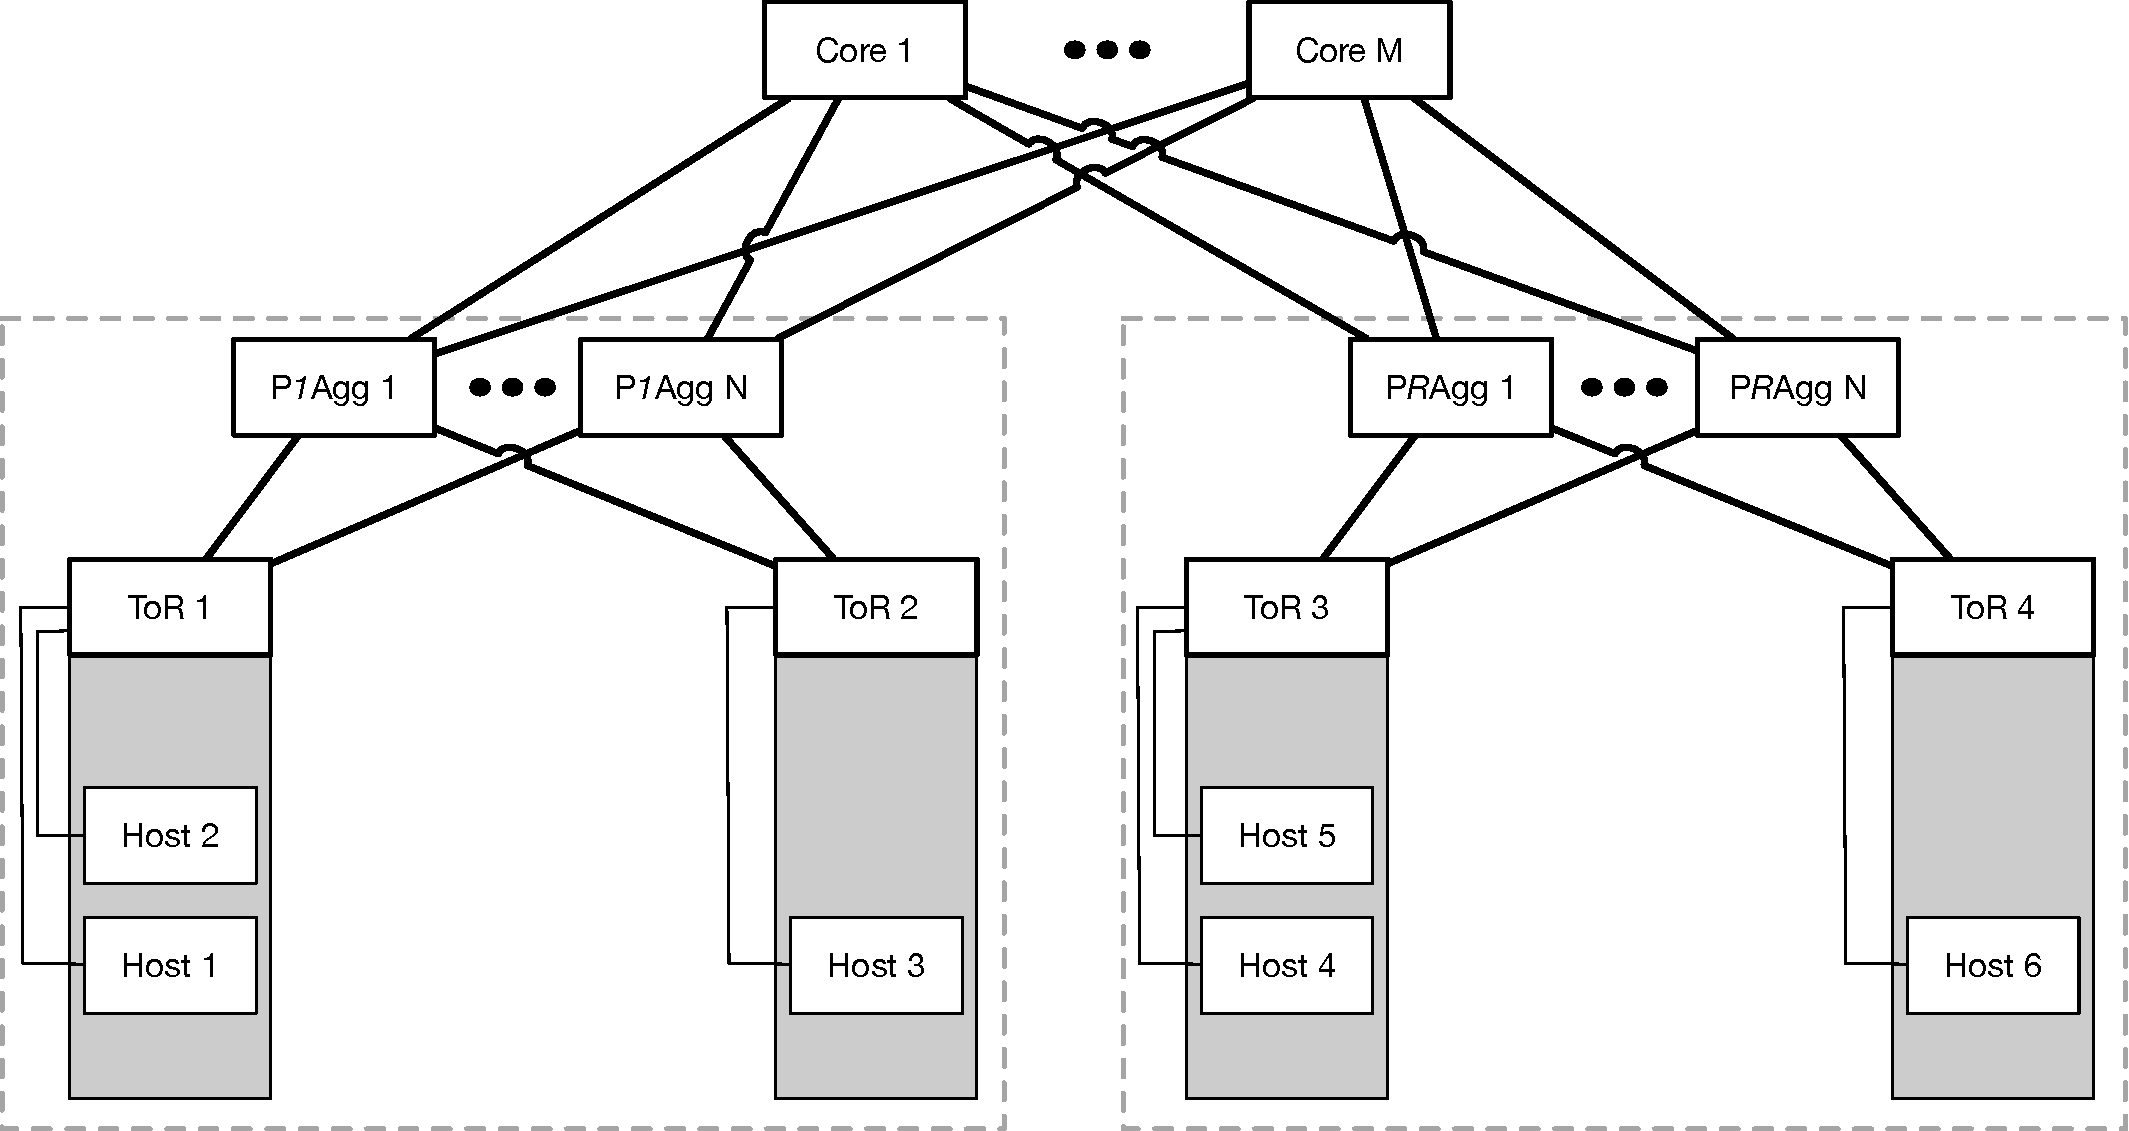
\includegraphics[width=0.4\paperwidth]{topology.pdf}


\section{Design}
\FIXME{diagram}
When to activate booster, and on which flows.
How to pair boosters together.

This interferes with load-balancing.
  Or how can load-balancing take failing links into account.

  background~\cite{Chen:2012:EEE:2182751.2182754}

How sensitive are we to topology, addressing schemes, and routing strategy (including load balancing) that might be in place to utilise fan-out or path diversity
(We don't want to get too involved in traffic diffusion, ideally, but can it be escaped?)




\section{Example: Network-layer FEC}

According to Zhuo et al~\cite{Zhuo:2017:UMP:3098822.3098849} corruption affects fewer links (2-4\% -- wrt congested links or total links?), but the effects are heavier, and the failure is stable over time, when compared with congestion.

They only look at switch-switch links: we do not have any data whether server
links are less likely to fail. Failures have low locality (not zero, because
of interconnection at switches). One of the surprising results of their
research is that failures can occur at any point of the hierarchy with the
same likelihood -- this despite the disparity in link lengths. Server links
are max 10 feet long, whereas cables from ToR to aggregation can be 10x
longer.

\paragraph{Placement} (on a limb) Target ToR since:
\begin{itemize}
  \item If the switch-ToR link fails, the whole rack (~30x links) are
    affected, whereas if a host-ToR link fails then that's a single link.
  \item Similarly, addressing between FEC-protected hosts is reduced by a
    factor of \~30, since we can make use of hierarchical addressing. This
    affects the number of problematic links we can mitigate against.
  \item Having host-level boosters would be very expensive, to purchase, power, and connect the boosters to each host. Rather than improve things for individual hosts at high expense, we seek improve things for racks at moderate expense.
\end{itemize}


Technical issues:
\begin{enumerate}
  \item Link-layer source quenching when boosting, rather than relying on higher-layer protocols (e.g., TCP's congestion control).
  \item Placement (Need to specify network topology early on.)
  \item How the system should react to packet reordering, and retransmissions.
  \item Can FEC (and other boosters) be done independently from load-balancing?
  \item Interaction of FEC with error correction in PHY.
  \item How many failed links does the system tolerate with given resources?
  \item To what extent is corruption reduced to congestion by this work?
  \item How interacts with multipath routing.
\end{enumerate}

We base our model on fat-tree topology~\cite{Al-Fares:2008:SCD:1402946.1402967}.
  involves a lot of cabling, opportunities for link faults


L2 network~\cite{PortLand} and label switching?    

ns-3 Model

\FIXME{Describe tagging format}

FEC in PHY/medium. Link-level + frame-level + erasure vs error correction.

What happens upon retransmission of TCP? Or are we able to eliminate retransmissions?


\section{Prototype implementation}
Some bits done in P4, and other bits that can co-/entirely run on FPGA or a host's CPU.

Streaming flits through SDNet block.

source quench and slack buffer, similar to Stop and Go in Myrinet~\cite{342015}.


\section{Evaluation}
\FIXME{table/graph}
Ultimately we'd like to show application-level service quality, but
network-level performance might be a pragmatic surrogate.

Generate traffic to saturate a 40G link.

Emulating packet loss and packet corruption -- can both these be done using a P4 program?

Showing the traffic makes it through $2 < H < 5$ hops in the presence of
network mishaps, and that application-level performance is sustained.
(As a control experiment, showing that non-boosted traffic leads to application degradation.)

\section{Related work}
Data centers:
Eden.
CorrOpt.
CONGA.
NaaS.
NetAgg.

Boosting elsewhere: JMS' work from the 90's.

\section{Conclusion}

\bibliographystyle{ACM-Reference-Format}
\bibliography{paper}

\end{document}
